\documentclass[11pt]{article}
\usepackage[top=1in, bottom=1in, left=1in, right=1in]{geometry}
\usepackage{amssymb}
\usepackage{physics}
\usepackage{url}

\usepackage{listings}
\lstset{frame = tb, language = Python,
		aboveskip = 3mm, belowskip = 3mm,
		tabsize = 3, columns = flexible,
		basicstyle = \small\ttfamily}

\usepackage{graphicx}
\graphicspath{{c:/Users/Jacob/Documents/Coding_Stuff/LaTeX/Honors_Thesis/Figures/}}

\usepackage{fancyhdr}
\pagestyle{fancy}
\renewcommand{\sectionmark}[1]{\markboth{#1}{}}
\fancyhf{}
\fancyhead[R]{\leftmark}
\fancyhead[L]{Monte Carlo and Lattice QCD}
\fancyfoot[C]{\thepage}
\fancypagestyle{plain}{\fancyhf{}
	\renewcommand{\headrulewidth}{0pt}}

\usepackage{tikz}
\usetikzlibrary{shapes.callouts}
\tikzset
{
	line/.style = {black},
	transition/.style = {dashed, black}
}

\begin{document}
\thispagestyle{empty}
\begin{center}
	\vspace*{1cm}
		
	\LARGE
	\textbf{Monte Carlo Applications and Lattice QCD}
		
	\vspace{2cm}
	\Large
	\textbf{Jacob Scott}
		
	\vspace{1cm}
	Advisor: Dr. Tom Blum
		
	\vspace{1cm}
	Spring 2016
		
	\vspace{1.5cm}
	\normalsize
	\textbf{Abstract}
\end{center}

The Monte Carlo method is a broad class of random sampling techniques. One facet of its power arises in its ability to compute complex multidimensional integrals simply through large sample sizes. In this paper, we explore the use of Monte Carlo techniques and their advantage in modeling physical statistical systems such as the Ising model, Feynman path integrals and lattice QCD. The Metropolis algorithm, one type of Monte Carlo method, is applied to evolve these systems while other methods are used to compute and measure different observables. What we will see is that these measurements are an accurate representation of the real-world counterpart whose error arises from simplifying assumptions made on the models, approximations of the measurements and the finite simple sizes. These above sources of error can be rectified by more accurate models and larger sample size, the former of which we will see in modeling of lattice QCD.

\break

\tableofcontents
\newpage

\section{Introduction}

The myriad methods developed in the sciences and mathematics, no matter how esoteric, come about due to a problem that is unsolved that scientists or mathematicians want to solve. Problems arise due to new information, new measurements or even just a new idea that one person may have and these problems are solved using one or a number of these methods or new methods are discovered.

The field of lattice quantum chromodynamics (QCD) is a good example of this. Lattice QCD is the study of the strong force through the use of discretized spacetime lattice simulations and is considered a nonperturbative theory. Because of this, more traditional methods can not be used. In electrodynamics, the coupling constant (the constant that determines the strength of the force) is the fine-structure constant:
\begin{align}
	\alpha=\frac{1}{4\pi\epsilon_0}\frac{e^2}{\hbar c}\approx\frac{1}{137}.
\end{align}
Because of its extremely small value, perturbative methods can be implemented and approximations can be made that are in the form of series of powers of $\alpha$. Such series would be dominated by the first couple terms and even first-order solutions can be very accurate. Whereas in QCD, the coupling constant $g$ is of the order of one and therefore perturbation theory is not a valid method for low energy systems but lattice QCD is. Lattice QCD is not perturbative but rather finds its power in the form of computers.

Lattice QCD is a discrete and numerical approximation of the continuum and as such, when the spacing between lattice sites $a\to0$, we return to the continuous theory. Because of this, the error that arises comes from this discretization and also from the numerical methods used in this paper. A common compromise is the choice for lattice size. Too large and the program can take too long to run to be practical. Too small and the error on the data is large. 

The numerical methods that are used in this paper are Monte Carlo methods. These methods rely on random sampling in the hopes that doing so will eventually approximate the equilibrium state of a system. The method used specifically in the evolution of the systems is the Metropolis algorithm, an algorithm that decides whether a change in the system should be accepted or rejected. This decision is based on the physics of the system. For example, if a system tends towards the lowest energy state, then the Metropolis algorithm is used to accept states that are a lower energy. Monte Carlo methods are also used to approximate multi-dimensional integrals to measure specific observables of a system. As such, this paper highlights the flexibility and power of the aforementioned methods and shows how measurements are relatively simple once a system is properly modeled.

In this paper, I will explore simpler systems using the methods I will then use for lattice QCD. These systems are the Ising model and the harmonic oscillator. In every simulation, the same methods are used with the only changes coming in the form of the physics of the specific systems. Even though these systems are vastly different, the methods are the same. Known methods, in this case Monte Carlo methods,  are used to explore a newer problem, nonperturbative QCD.

\section{Monte Carlo and the Metropolis Algorithm}
The Monte Carlo method is a broad class of computational algorithms where the use of random sampling yields numerical results. Any problem that has a probabilistic interpretation can be solved with the Monte Carlo method. And, due to the law of large numbers, with a sufficiently large sample size, expectation values (or, analogously, any integral) can be approximated by a simple mean. For example, we can approximate the following integral by \cite{MonteCarloLLN}:
\begin{align}
	\int_a^bf(x)\dd{x}=\frac{b-a}{N}\sum_{i=1}^Nf(x_i)
\end{align}
for $N$ samples. This integral can be generalized to any finite dimensional integral over some volume $\Omega$ as
\begin{align}
	\int_\Omega f(x)\dd{x}=\frac{V(\Omega)}{N}\sum_{i=1}^Nf(x_i)
	\label{eq:MCIntGen}
\end{align} where $V(\Omega)$ is the volume of $\Omega$. This is valid for any dimension and has little effect on computational time. In this paper, high dimensional integrals are computed numerically and so this method holds an advantage.

\subsection{Markov Chain}
A Markov chain is a sequence of states $(x_0,\ x_1,\ldots,\ x_n)$ such that any state $x_{i+1}$ depends only on its immediately proceeding state $x_i$, a property called memorylessness. The probability of the transition from state $x_i$ to state $x_{i+1}$ is the transition amplitude and defining such a function allows for the modeling of a Markov chain. Every model in this paper has the property of memorylessness and can be modeled as a Markov chain.

Moreover, every model can be modeled by Markov chain Monte Carlo methods. The equilibrium of a many-state system can be difficult, if not impossible, to solve. Rather, starting with an initial state $x_0$, the system will fall into equilibrium, or reach the target distribution, at state $x_n$ for some $n$ large enough. This is true because the algorithms in this paper maintain detailed balance and ergodicity so these algorithms will, eventually, converge to the correct probability distribution. The initial state $x_0$ is arbitrary although a guess of the equilibrium distribution is helpful so as to converge quicker. Beforehand, the equilibrium distribution is unknown but it can be approximated by evolving the Markov chain until the resulting distribution satisfies within an error the conditions of the equilibrium state. As stated before, there is a transition amplitude between states $x_i$ and $x_{i+1}$. So, for some change on $x_i$, a decision must be made whether it will change to $x_{i+1}$ or not change. The method used in this paper is called the Metropolis algorithm.

\subsection{Metropolis Algorithm}
For a Markov chain, there is a probability density $f(x_j|x_i)$ of choosing state $x_j$ as the next candidate in the Markov chain given state $x_i$. The change in $x_j$ from $x_i$ is usually small. This is to allow for a large number of accepted changes but it isn't too small so as to not change the state negligibly. There is also the conditional probability $P(x_j|x_i)$ of changing to state $x_j$ given state $x_i$. If we assume the process is reversible \cite{MonteCarloMetropolis}, then it satisfies the condition of detailed balance
\begin{align}
	q(x_j|x_i)P(x_i)=q(x_i|x_j)P(x_j)
\end{align}
where $P(x)$ is the desired probability distribution and $q(x_j|x_i)$ is the transition amplitude from $x_i$ to $x_j$. Noting that $q(x_j|x_i)=f(x_j|x_i)P(x_j|x_i)$, this can be rewritten as
\begin{align}
	\frac{P(x_j|x_i)}{P(x_i|x_j)}=\frac{f(x_i|x_j)q(x_j)}{f(x_j|x_i)q(x_i)}.
	\label{eq:MetAlRat}
\end{align}
We wish to find the probability $P(x_j|x_i)$ that satisfies equation \ref{eq:MetAlRat}. The Metropolis choice is
\begin{align}
	P(x_j|x_i)=\min\left(1,\ \frac{f(x_i|x_j)P(x_j)}{f(x_j|x_i)P(x_i)}\right).
	\label{eq:TransAmp}
\end{align}
Thus, the probability of changing from state $x_i$ to state $x_j$ is shown in equation \ref{eq:TransAmp}. The Metropolis steps are as follows:
\begin{enumerate}
\item Initialize the system with some initial state $x_0$.
\item Randomly pick a state $x_j$ with probability given by $f(x_j|x_i)$ where $x_i$ is the current state.
\item Accept this new state with probability $P(x_j|x_i)$ as given in equation \ref{eq:TransAmp}.
\item If accepted, change the state from $x_i$ to $x_j$.
\item Otherwise, keep the state $x_i$.
\item Repeat steps 2-5.
\end{enumerate}
For the models in this paper, a uniform distribution is used for choosing a new state $x_j$, thus $f(x_j|x_i)=f(x_i|x_j)$. Equation \ref{eq:TransAmp} can be rewritten as shown in \cite{MonteCarloMetropolis} as
\begin{align}
	q(x_j|x_i)=\min\left(1,\ \frac{P(x_j)}{P(x_i)}\right).
\end{align}
From the above equation, we can see that if the probability of state $x_j$ is equal to or greater than the probability of $x_i$ (i.e. the new state is more likely in the equilibrium distribution than the old state), then the change is automatically accepted. Thus acceptance of a new state occurs with certainty when $P(x_{new})\geq P(x_{old})$. This can once more be rewritten in a piecewise fashion as
\begin{align}
P(x_{i+1}|x_i)=\begin{cases}
\quad\ 1\qquad&\text{if}\ \ \displaystyle{\frac{P(x_{i+1})}{P(x_i)}\geq1}\\
\displaystyle{\frac{P(x_{i+1})}{P(x_i)}}\qquad&\text{otherwise.}\\
\end{cases}
\end{align}
The functions for $P(x_i)$ will be defined later in the paper for the specific models.
%g
The Metropolis algorithm allows for the evolution of a statistical system without necessarily the knowledge of the desired probability distribution. But Monte Carlo can also be used in the measurement of observables of the system; after all, not much use is gained by modeling a system if no measurements are made on it.

\subsection{Monte Carlo Measurements}
As shown in equation \ref{eq:MCIntGen}, Monte Carlo has its uses in the numerical integration of multi-dimensional integrals. We will see that the latter two models in this paper are derived from the Feynman path integral which is, essentially, an infinite dimensional path integral which accounts for every possible path from one state to another (since in quantum mechanics, every path will have a nonzero probability due to effects such as tunneling).

When discretized, any integral is approximated by a sum. We will see that for some expectation average $\langle f(x)\rangle$ that is weighted by some probability density function $g(x)$, it can be written as
\begin{align}
	\langle f(x)\rangle=\int f(x)g(x)\dd{x}.
\end{align}
But if some $x$ has a probability of being chosen proportional to $g(x)$, then the unweighted, simple average
\begin{align}
	\langle f(x)\rangle\approx\overline{f(x)}=\frac{1}{N}\sum_{i=1}^Nf(x_i)
	\label{eq:MCExp}
\end{align}
can be used as an approximation by \cite{MainPaper}. The term $\overline{f(x)}$ is the Monte Carlo estimator for $\langle f(x)\rangle$. Since $N$ is finite, the estimator will never be exact. In the limit, $\overline{f(x)}\to\langle f(x)\rangle$ as $N\to\infty$. This result allows for the approximation of any expectation value where the error is dependent on $N$.

\section{The Ising Model}
The Ising model is a good place to begin with the Metropolis algorithm because of its simplicity. On the lattice for the Ising model, the interaction is nearest-neighbor and discrete. For each lattice site $k$, there is a corresponding spin $s_k\in\{-1,1\}$. Given this, the Hamiltonian for the Ising model is
\begin{align}
	H=-\sum_{\langle i,j\rangle}J_{i,j}s_is_j+h\sum_js_j
\end{align}
where $J_{i,j}$ is the interaction strength between neighbors at site $i$ and site $j$ and $h$ is an external magnetic field. If we assume no external magnetic field and a constant interaction strength, then we obtain
\begin{align}
	H=-J\sum_{\langle i,j\rangle}s_is_j.
	\label{eq:Energy}
\end{align} Since each site has two possibilities, for a $d$-dimensional hypercube with side length $n$, there are $2^{n^d}$ possibilities for the lattice. This is the advantage of using Monte Carlo techniques. Many measurements of the lattice can be made to simulate the model and derive an accurate evolution on which observables can be measured. In the case for the Ising model, and subsequent models, the Metropolis algorithm is used.

\subsection{Application of the Metropolis Algorithm}

For the evolution of the Ising model, one must decide whether a change in the lattice should occur or not. The Metropolis algorithm gives the probability $P(\vb{x}_{\ell+1}\mid \vb{x}_\ell)$ for a transition from state $x_\ell$ to $x_{\ell+1}$. If the change in energy $\Delta H$ is less than zero, then the change at the site will occur since the system tends towards a lowest energy state. Otherwise, the transition probability follows the Boltzmann distribution $e^{-\beta\Delta H}$ where $\beta=1/k_BT$ \cite{IsingModelBook}. Thus, the Metropolis transition probability is
\begin{align}
	P(\vb{x}_{\ell+1}\mid \vb{x}_\ell)=
	\begin{cases}
		e^{-\beta\Delta H},\quad&\text{if }\Delta H>0\\
		1,&\text{otherwise.}
	\end{cases}
	\label{eq:ProbIsing}
\end{align}
To obtain the change in energy $\Delta H$, a new state must be chosen for the lattice site. In the case of the Ising model, there are only two states: $\pm1$. Therefore, the new energy is just the opposite sign of the old energy according to equation \ref{eq:Energy}. Thus, the change in energy at lattice site $j$ is double the original energy at that site, or
\begin{align}
	\Delta H_j=-2Js_j\sum_is_i.
	\label{eq:DeltaH}
\end{align}
So the change in energy can be calculated this way since the new spin being chosen for site $j$ is implicit in the equation. For later simulations, this is not the case and so a slightly different state is chosen randomly to calculate the change induced by the new state. Now to apply this, the steps for the evolution of the Ising model are as follows:
\begin{enumerate}
\item Choose a lattice site $j$.
\item Calculate the change in energy $\Delta H_j$ at the site $j$.
\item If $\Delta H<0$ then change the spin at site $j$.
\item Otherwise assign it a probability $\exp(-\beta\Delta H_j)$ of changing.
\item Repeat steps 1-4 for every site on the lattice.
\end{enumerate}

This completes one sweep of the lattice as every site on the lattice is checked to flip. Step 4 can be completed by randomly choosing a number $a\in[0,1]$ such that if $a<\exp(-\beta\Delta H)$ the change occurs otherwise the change is rejected.

A problem faced by virtue of a finite lattice is the boundary. In this model, the boundary lattice sites are missing neighbors due to the limitations of a computer simulation. One solution to this problem, which is used in the simulations in this paper, is periodic boundary conditions. The missing neighbors of the boundary sites are replaced by the sites on the opposite side of the lattice.

\begin{figure}[ht]
\centering
\begin{tikzpicture}
	\draw[gray, thick,] (0,2) -- (0,-2);
	\draw[gray, thick] (2,0) -- (-2,0);
	\filldraw[black] (0,0) circle (1.5pt);
	\node[above] at (0,2) {\footnotesize($x$, $(y+1)\text{mod}N$)};
	\node[right] at (2,0) {\footnotesize($(x+1)\text{mod}N$, $y$)};
	\node[below] at (0,-2) {\footnotesize($x$, $(y-1)\text{mod}N$)};
	\node[left] at (-2,0) {\footnotesize($(x-1)\text{mod}N$, $y$)};
	\node[below right] at (0,0){\footnotesize($x$, $y$)};
\end{tikzpicture}
\caption{Neighboring sites of site $(x,y)$ with periodic boundary conditions} \label{fig:PBC}
\end{figure}

For example, on a square 2-dimensional lattice with sides $N$, the neighbors of any site $(x,y)$ will be as shown in figure \ref{fig:PBC} where mod represents the modulo operator. As long as the interactions are shorter than the lattice size, then the lattice is effectively infinite for each point. The interactions for the Ising model are nearest-neighbor, so periodic boundary conditions are applied for the boundary sites.

\subsection{Measurements on the Lattice}
\subsubsection{Magnetization}
Now with the ability to model the Ising Model, measurements can now be made. It is helpful to note that dimensionality has so far been arbitrary with exception to the remarks on figure \ref{fig:PBC}. For $d$ dimensions, for each lattice site $(x_1,x_2,\ldots,x_d)$, it would have $2d$ neighbors for measurement of the change in energy. One measurement is magnetization given by
\begin{align}
	M=\sum^{N^2}_{j=1}s_j
\end{align}
and the magnetization per spin is just $m=M/L^2$. What should be expected for the magnetization of this system?

From equation \ref{eq:ProbIsing}, one can see there are just two parameters: the temperature $T$ and the interaction strength $J$. But these can just be written as one parameter $T_J=J/k_BT_c$ (with the Boltzmann constant included) since they have the same effect on $\Delta H$. At some point, the system will reach an equilibrium where $m$ will oscillate about some value. Because $T_J>0$, the interactions are ferromagnetic and so spins will tend to align in the same direction. This is seen at low $T$ since the thermal energy is not large enough to overcome the alignment. Therefore, the lattice will be highly ordered with $\abs{m}\approx1$ or slightly less. But with high $T$, the magnetic interactions will be dominated by the thermal energy and neighboring spins will not be correlated; so $m\approx0$. There is some temperature at which the thermal energy is larger than the magnetic interactions of the lattice sites. This is the critical temperature $T_c$.
\begin{figure}[ht]
\begin{lstlisting}
def Ising2D(lattice, Jkbt, N):
    magnetization = 0

    for p in product(range(N), range(N)):
        i, j = p
        energy = (lattice[i][(j - 1) % N] + lattice[i][(j + 1) % N] +
                   lattice[(i - 1) % N][j] + lattice[(i + 1) % N][j]) *
                   lattice[i][j]
        magnetization += lattice[i][j]

        if energy <= 0 or np.random.random() < np.exp(-2 * Jkbt * energy):
            lattice[i][j] *= -1

    return lattice, magnetization
\end{lstlisting}
    \caption{Python code for one sweep of a $N$x$N$ lattice with $T_J=\texttt{Jkbt}$. The change in energy, $\Delta H$, for a site is calculated and stored in \texttt{energy} where then a Metropolis update is performed. Also, the magnetization at that site is stored in \texttt{magnetization} and is used later to determine the equilibrium magnetization of the lattice. This is carried out for every site on the lattice, then returning the updated lattice and its total magnetization.} \label{fig:Ising2DCode}
\end{figure}

In figure \ref{fig:Ising2DCode}, the function that completes one sweep of the lattice is shown. Each lattice site is checked to change before the next site is checked. The \texttt{product} function in the for loop creates tuples whose values are stored in \texttt{i} and \texttt{j} for each loop thus completing the sweep row by row. If the energy change is accepted according to the if statement, the spin value at the lattice site is flipped. It is important to note that the lattice must be thermalized before measurements can be taken, that is the lattice must first reach an equilibrium. This is done by completing enough lattice sweeps before taking measurements. The Ising model simulations discussed are done with 10000 sweeps and only the latter fourth of sweeps are measured. The application of this function is shown in its entirety in the appendix. 

For the parameter $T_J$, the critical temperature is at $T_J=\frac{1}{2}\ln(1+\sqrt{2})$ \cite{IsingModelBook}. In figure \ref{fig:MvTdN}, the behavior of different temperatures on different lattice sizes is shown. The absolute magnetization is measured instead of the signed magnetization because the magnetization at which a specific lattice settles to can be either $\pm x$ for $x\in[0,1]$ and the magnetization can rarely but suddenly switch signs due to finite size of the lattice. Ignoring the sign fixes these issues and the result is shown in figure \ref{fig:MvTdN}; for low $T$, the lattice is more ordered and the absolute magnetization is near 1. For high $T$, the magnetization oscillates about 0 as discussed above. Since the absolute value of the magnetization is measured, the values plotted for high temperature represent the magnitude of these oscillations. For the smaller lattice size (e.g. $N=5$), the oscillations will be larger since each site will have a greater impact on the total magnetization of the lattice.

\begin{figure}[h]
	\centering
\includegraphics[scale=0.60]{Mag_vs_T_Different_N.png}
	\caption{The normalized magnetization plotted against temperature with respect to the critical temperature for various lattice sizes. The values were computed by evolving the lattice until equilibrium, then computing the average for many measurements of the magnetization.}
	\label{fig:MvTdN}
\end{figure}

\subsubsection{Susceptibility}

Susceptibility can also be measured on the lattice. It is the measure of the change in magnetization due to a magnetic field. The effect of lattice size and temperature on magnetic susceptibility $\chi$ can also be measured by \cite{IsingSus}
\begin{align}
	\chi&=\pdv{\langle M\rangle}{H}\\
	&=\frac{1}{T}(\langle M^2\rangle-\langle \abs{M}\rangle^2).
	\label{eq:Sus}
\end{align}
This measurement only requires the average magnetization, which is already measured, and the average of the squared magnetization. In the simulation for figure \ref{fig:MvTdN}, the susceptibility was also measured using equation \ref{eq:Sus} as shown in figure \ref{fig:SvTdN}. A large susceptibility occurs where there is a large standard deviation in the magnetization of the sweeps (the susceptibility is the variance of the magnetization). At low $T$, the lattice is in equilibrium at some magnetization and at high $T$, the lattice is unordered and so the magnetization does not vary far from 0. In either case, the variance is small. At $T=T_c$, the lattice does not reach an equilibrium and so the change in magnetization is large accounting for the large peak in figure \ref{fig:SvTdN}.

\begin{figure}[h]
	\centering
\includegraphics[scale=0.60]{Sus_vs_T_Different_N.png}
	\caption{The normalized susceptibility for the same simulation as figure \ref{fig:MvTdN}.}
	\label{fig:SvTdN}
\end{figure}

The Metropolis algorithm allowed us to model an Ising model system. With a model, measurements can be made on the system; the measurement of magnetization dependent on the parameters of the system was done above. Other measurements such as specific heat or correlation length can be made. Also, a variable interaction strength, nonzero external magnetic field or a higher dimensional model can have significant changes on the system with little change to the program. Going forward, the Monte Carlo method and the steps of the Metropolis algorithm used here will be applied for more complicated systems, specifically with respect to the discretized version of the Feynman path integral.

\section{The Feynman Path Integral on the Harmonic Oscillator}
\subsection{Derivation}
In a classical system, a path a particle will take in a potential field is determined by the principle of least action. This states that the action which can be written as a function 
\begin{align}
	S[x]=\int_{t_i}^{t_f}\mathcal{L}(\vb{x},\dot{\vb{x}})\dd{t},
	\label{eq:Action}
\end{align}
where $\mathcal{L}(x,\dot{x})$ is the Lagrangian, gives the path of the particle when the action reaches a minimum. Classically, there is a unique path for a particle but quantum mechanically, due to its probabilistic nature, every path is possible and must be accounted for in calculations. With this in mind, how does one find the probability to go from $(x_i,t_i)$ to $(x_f,t_f)$ in some potential field when all paths are possible?

We start with the propagator in wave mechanics given by \cite{QuantumBook}

\begin{align}
	K(\vb{x}_f,t_f;\vb{x}_i,t_0)=\sum_a\bra{\vb{x}_f}\ket{a}\bra{a}\ket{\vb{x}_i}\exp\left[\frac{-iE_a(t_f-t_0)}{\hbar}\right]
\end{align}
which can be found as an integral operator for a wave function $\psi(\vb{x_f},t_f)$ acting on the initial wave function:
\begin{align}
	\psi(\vb{x}_f,t_f)=\int\dd[3]{x}K(\vb{x}_f,t_f;\vb{x}_i,t_0)\psi(\vb{x}_i,t_i).
	\label{eq:WavFuncProp}
\end{align}
The propagator can be rewritten as

\begin{align}
	K(\vb{x}_f,t_f;\vb{x}_i,t_0)=\mel{\vb{x}_f}{\exp\left[\frac{-iH(t_f-t_0)}{\hbar}\right]}{\vb{x}_i}.
	\label{eq:PropExp}
\end{align}
In both equations \ref{eq:WavFuncProp} and \ref{eq:PropExp} and as hinted by the name, the propagator can be interpreted as a time-evolution operator on an initial state $(\vb{x}_i,t_i)$ to a final state $(\vb{x}_f,t_f)$. This can ultimately be seen by
\begin{align}
\begin{split}
	K(\vb{x}_f,t_f;\vb{x}_i,t_0)&=\sum_a\bra{\vb{x}_f}\ket{a}\bra{a}\ket{\vb{x}_i}\exp\left[\frac{-iE_a(t_f-t_0)}{\hbar}\right]\\
	&=\mel{\vb{x}_f}{\exp\left[\frac{-iH(t_f-t_0)}{\hbar}\right]}{\vb{x}_i}\\
	&=\bra{\vb{x}_f,t_f}\ket{\vb{x_i},t_i}.
\end{split}
\end{align}
The Feynman path integral gives us a way to calculate the propagator. It is as follows from \cite{MainPaper}:

\begin{align}
	\bra{x_f,t_f}\ket{x,t_i}=\int\mathcal{D}[x(t)]e^{iS[x]/\hbar}
	\label{eq:ContPathInt}
\end{align}
where the position operators have been simplified to one dimension although the generalization for higher dimensions is analogous.

In equation \ref{eq:ContPathInt}, $\mathcal{D}[x(t)]$ represents all paths that the particle can take and is weighted by the $e^{iS[x]/\hbar}$ term. One concern is the divergence of the integral; it is an infinite dimensional integral with nonzero contributions from each dimension. But the integral will not diverge. Since for paths far from the classical path, the action will be large yielding a large frequency and thus a large phase shift compared to paths close to it. This will deconstructively interfere with other paths far from the classical path thus contributing little to the integral. Also at the classical $\hbar\to0$ limit, the same behavior will be seen and the only surviving path is the one with a minimized action.

It is more convenient to work in Euclidean space so a change of variables $t\to it$ by a Wick rotation allows for simpler calculations for computers but does not effect the physics. Furthermore, using natural units such that $\hbar=c=1$, the above equation is further simplified. This will give
\begin{align}
	\bra{x_f,t_f}\ket{x,t_i}=\int\mathcal{D}[x(t)]e^{-S[x]}
\end{align}	
where one can see that both paths far from the classical path contribute little and the $\hbar\to0$ limit still holds true due to the exponential dampening.

\subsection{Discretization}
The above equation is called the propagator which gives us complete information about the system. To solve this path integral numerically, the propagator must be discretized. To do so, we can split the possible paths of the particle into $N-1$ time slices such that for one path, the particle will travel along $(x_1,t_1),\ldots,(x_N,t_N)$ \cite{QuantumBook}. Thus the previously infinite dimensional integral can be approximated as
\begin{align} 
	\int\mathcal{D}[x(t)]=A\underbrace{\int_{-\infty}^{\infty}\ldots\int_{-\infty}^{\infty}}_{N-1\ \text{integrals}}\dd{x_1}\ldots\dd{x_{N-1}}
\end{align}
where $A$ is a normalization constant. Using this, we can write
\begin{align}
\begin{split}
	&\bra{x_f,t_f}\ket{x,t_i}\\
	&\qquad\ =A\int_{-\infty}^{\infty}\ldots\int_{-\infty}^{\infty}\dd{x_1}\ldots\dd{x_{N-1}}e^{-S[x_1]}\ldots e^{-S[x_{N-1}]}\\
	&\qquad\ =A\int_{-\infty}^{\infty}e^{-S[x_1]}\dd{x_1}\ldots\int_{-\infty}^{\infty}e^{-S[x_{N-1}]}\dd{x_{N-1}}.
\end{split}
\end{align}
This discretization also effects the action. From equation \ref{eq:Action}, writing the Lagrangian as $\frac{1}{2}m\dot{x}^2-V(x)$ and focusing only on the $j$th time slice, we have 
\begin{align}
	S[x_j]&=\int_{t_j}^{t_{j+1}}\frac{m\dot{x}^2}{2}+V(x)\dd{t}\\
	&=\Delta t\left[\frac{m}{2}\left(\frac{x_{j+1}-x_j}{\Delta t}\right)^2+\frac{1}{2}(V(x_{j+1})+V(x_j))\right]
	\label{eq:ActionDiscrete}
\end{align}
where $\Delta t$ is the length of each time slice or $\Delta t=\frac{t_f-t_i}{N}$. The energies are summed because of the change from Minkowski to Euclidean space; a factor of $i^2$ comes from the kinetic term and the minus signs are factored out, effectively changing the Lagrangian into a Hamiltonian.  Because time is discrete, the integral can be solved just by evaluating the endpoints which yields equation \ref{eq:ActionDiscrete}. Summing over all $N-1$ time slices, we obtain the action contribution from every path. Therefore,
\begin{align}
	\bra{x_f,t_f}\ket{x,t_i}=A\int_{-\infty}^{\infty}\dd{x_1}\ldots\int_{-\infty}^{\infty}\dd{x_{N-1}}e^{-S[x]}
	\label{eq:PathIntNum}
\end{align}
where
\begin{align}
	S[x]=\sum_{j=0}^{N-1}\left[\frac{m}{2\Delta t}(x_{j+1}-x_j)^2+\Delta tV(x_j)\right].
	\label{eq:ActionTot}
\end{align}

In equation \ref{eq:PathIntNum}, the contribution of paths are exponentially damped so quantum mechanical paths (paths far from the classical path) contribute very little to the path integral because of their low probability. The path integral has now been discretized in terms of $N-1$ time slices where, for each slice, the action is assumed to be constant. So as $\Delta t\to0$, equation \ref{eq:ContPathInt} is recovered.

It is important to note that if $\Delta t$ is large and $T=t_f-t_i$, then the propagator can be rewritten as
\begin{align}
	\mel{x}{e^{-HT}}{x}\approx e^{-E_0T}\abs{\bra{x}\ket{E_0}}^2
\end{align}
since the ground state dominates due to the exponential. So assuming a large $\Delta t$, the propagator is effectively measured for the ground state wave function \cite{MainPaper}. Shown below, $\Delta t$ is taken to be 1/2 and $N=8$, so then $T=4$.

\subsection{Ground State Harmonic Oscillator}
The integral was computed for a one-dimensional harmonic oscillator with
\begin{align}
V(x)=\frac{x^2}{2},\ \ A=\left(\frac{m}{2\pi a}\right)^{N/2}\ \ \text{and}\ \ \Delta t=\frac{1}{2}.
\end{align}
The mass was set at $m=1$ and the dimension of the integral was set at $N=8$. 

The integral was computed using Mathematica as shown in figure \ref{fig:QHO}. The blue line represents an analytic approximation of the solution. As $N$ gets large, this numerical approximation will become more accurate but at the cost of computing power  which is a common theme in numerical techniques. 
\begin{figure}[h]
	\centering
	\includegraphics[trim={0 0.7cm 0 0}]{Quantum_Oscillator_Path_Integral.pdf}
	\caption{Plot of $\mel{x}{e^{-Ht}}{x}$ for various values of $x$ calculated using equations \ref{eq:PathIntNum} and \ref{eq:ActionTot}. The blue line represents the analytic solution where $\mel{x}{e^{-H\Delta t}}{x}\approx\abs{\bra{x}\ket{E_0}}^2e^{-E_0\Delta t}$ and $\bra{x}\ket{E_0}=\exp(-x^2/2)/\pi^{1/4}$.}
	\label{fig:QHO}
\end{figure}

\subsection{Monte Carlo Application}
The above derivation is in regards to the ground state of the system. In systems such as those found in quantum field theory, the ground state is a vacuum and the measurement of observables in excited states is desired. The vacuum expectation value $\expval{x(t_2)x(t_1)}{0}$ can be written as the correlation function \cite{CorrFunctions}
\begin{align}
	\langle x(t_1)x(t_2)\rangle=\frac{\int \mathcal{D}[x(t)]x(t_2)x(t_1)e^{-S[x]}}{\int \mathcal{D}[x(t)]e^{-S[x]}}
	\label{eq:CorFunction}
\end{align}
where $t_i<t_1<t_2<t_f$. Notice that equation \ref{eq:CorFunction} is written in the Heisenberg picture; the operators are time-dependent (in this case the position operators). If we change to the Schr\"odinger picture, this equation can be rewritten keeping in mind the rotation to Euclidean time as
\begin{align}
	\langle x(t_1)x(t_2)\rangle&=\frac{\int\dd{x}\mel{0}{e^{-H(t_f-t_2)}}{x}\mel{x}{e^{-H(t_2-t_1)}}{x}\mel{x}{e^{-H(t_1-t_i)}}{0}}{\int\dd{x}\mel{0}{e^{-H(t_f-t_i)}}{0}}.\\
	\intertext{The numerator can be seen as an interruption on equation \ref{eq:ContPathInt} with the position operator $x$ at $t_1$ and $t_2$. Simplifying, we have}
	&=\frac{\int\dd{x}\mel{0}{e^{-H(t_f-t_2)}xe^{-H(t_2-t_1)}xe^{-H(t_1-t_i)}}{0}}{\int\dd{x}\mel{0}{e^{-H(t_f-t_i)}}{0}}.\\
	\intertext{A further simplification can be made by inserting the the complete set of states $\sum_i\ket{E_i}\bra{E_i}=1$ twice for $i=m,n$ next to the vacuum bra and ket. Letting $T=t_f-t_i$ and $t=t_2-t_1$, this ultimately yields \cite{MainPaper}}
	&=\frac{\sum_ne^{-E_nT}\mel{E_n}{xe^{-(H-E_n)t}x}{E_n}}{\sum_ne^{-E_nT}}.
\end{align}
Making the assumption that $T$ is large and $T\gg t$, the first term will dominate due to the exponential and we end up with
\begin{align}
	\langle x(t_1)x(t_2)\rangle=\mel{E_0}{xe^{-(H-E_0)t}x}{E_0}.
\end{align}

For the harmonic oscillator, if a complete set of states is inserted, only the $E_1$ states survive and thus we have
\begin{align}
	\langle x(t_1)x(t_2)\rangle&=\mel{E_0}{x}{E_1}\mel{E_1}{e^{-(H-E_0)t}}{E_1}\mel{E_1}{x}{E_0}\\
	&=\abs{\mel{E_0}{x}{E_1}}^2e^{-(E_1-E_0)t}
\end{align}
where we can now find the difference $E_1-E_0$. There is the unknown transition amplitude matrix element but if we let $G(t)=\langle x(t_1)x(t_2)\rangle$, then
\begin{align}
	E_1-E_0=\frac{1}{a}\log\left[\frac{G(t)}{G(t+a)}\right].
	\label{eq:ExciteE}
\end{align}
The quantity $G(t)$ can be considered as a weighted average from equation \ref{eq:CorFunction} with the weight being the exponential $\exp(-S[x])$. As stated in the first section, if the probability of the paths being drawn is proportional to this weight and the number of paths is large, then the weighted average can be approximated with an unweighted average. This means that
\begin{align}
	G(t)=\langle x(t_1)x(t_2)\rangle\approx\frac{1}{N}\sum_{n=1}^Nx_n(t_1)x_n(t_2).
	\label{eq:GApprox}
\end{align}

We now have everything needed to write a Metropolis algorithm program to generate an ensemble of paths. The process is analogous to the Ising model but with one exception: the value a site (or, in this case, a time slice) may have is not limited to only either $+1$ or $-1$ (as with the Ising model). Rather, a small random number $\alpha$ is added to the time slice to determine if such a change will be accepted by the Metropolis algorithm. Below are the steps to generate one path:
\begin{enumerate}
\item Choose a site $j$ in path $x$.
\item Add a random number $\alpha\in(-\epsilon,\epsilon)$ to the site $x_j$ so that $x_j\to x_j+\alpha$.
\item Calculate the change in action $\Delta S$ due to the change in $x_j$.
\item If $\Delta S<0$, then change the spin at site $j$.
\item Otherwise assign it a probability $\exp(-\Delta S)$ of changing.
\item Repeat steps 1-5 for every site on the path.
\end{enumerate}
The change in action can be written as
\begin{align}
	\Delta S= \frac{\alpha}{a}\left[(a^2+2)x_j+\left(\frac{\alpha^2}{2}+1\right)\alpha-x_{j+1}-x_{j-1}\right]
\end{align}
and, as with the Ising model, periodic boundary conditions are used, so the modulus operator is implied for $x_{j+1}$ and $x_{j-1}$. Figure \ref{fig:PathCode} shows the code that applies the steps above.
\begin{figure}[h]
\begin{lstlisting}
def dS(j, alpha):
    deltaS = (alpha / a) * ((a**2 + 2)*x[j] + (a**2/2 + 1)*alpha
    				 - x[(j + 1) % N] - x[(j - 1) % N])
    return deltaS

def update(x):
    for j in range(N):
        alpha = np.random.uniform(-eps, eps)
        deltaS = dS(j, alpha)        
        if deltaS < 0 or np.random.random() < np.exp(-deltaS):    
            x[j] += alpha
\end{lstlisting}
    \caption{Python code for one configuration of a path split into $N$ slices.}
\label{fig:PathCode}
\end{figure}

A few details must be brought up before making measurements as discussed in \cite{MainPaper}. The first is the starting configuration. An initial configuration should be used that is close to the equilibrium. This allows the program to reach equilibrium quicker. A initial configuration of $x_j=0$ for all $j$ is used in this program. One detail is the value of $\epsilon$. This number determines the maximum at which a site can change and there are pros and cons to having both a large or small $\epsilon$. If $\epsilon$ is small, many changes will be accepted but each successive path will be highly correlated. On the other extreme, successive paths will not be very correlated but changes will rarely be accepted. Therefore an $\epsilon$ is chosen by trial and error and $\epsilon=1.4$ is used in this code. Correlated paths are not desirable because the evolution of the path should be independent of previous values of the path. Therefore, not every path created is kept; for this model, every $N_{cor}$th path is recorded where $N_{\text{cor}}=20$. This number is inversely proportional to the lattice spacing $a$ and goes roughly as $N_{\text{cor}}\propto 1/a^2$. In this model, $a$ is large ($a=1/2$), so the choice of $N_{\text{cor}}$ is appropriate. Lastly, the paths must be thermalized before measurements are taken. In other words, the system must reach an equilibrium before paths are recorded and correlation functions measured. The appropriate number for this can also be measured by trial error. Here, $5N_{\text{cor}}$ paths are thrown away before measurements are taken.

\subsection{Measurements}
The quantity $G(t)$ can be measured numerically by using equation \ref{eq:GApprox} since the measurement is a simple product but other correlation functions could be calculated  and used by changing that which is used in the function \texttt{computeG} in figure \ref{fig:ComputeG}. The potential (in this case, that of the harmonic oscillator) can also be changed in the function \texttt{dS} in figure \ref{fig:PathCode}.

\begin{figure}
\begin{lstlisting}
def computeG(x, n):
    g = 0
    for j in range(N):
        g += x[j] * x[(j + n) % N]
    return g / N

def MCPaths(G):
    for i in range(N_cf):
        for j in range(N_cor):
            update(x)

        for k in range(N):
            G[i][k] = computeG(x, k)
\end{lstlisting}
\caption{Python code for calculating the correlation function $G(t)$ assuming it as an unweighted average. The measurement made on the paths is made only after every \texttt{N\_cor} paths and the \texttt{N} slices of each path in stored in the $i$th element of the array \texttt{G}.}
\label{fig:ComputeG}
\end{figure}

\subsubsection{Correlation Function}
The correlation function requires the correlation between each pair of sites on the path to be measured for each path. This is shown in figure \ref{fig:ComputeG}. For this code, 10000 paths are created and, to save computing time, binned into 100 different bins. Binning the paths does not change the statistics of the system, but makes calculations much quicker. Since $G(t)$ measures the correlation of two sites on the path and is the sum of a decreasing and an increasing exponential, we expect to see a curve similar to a hyperbolic cosine due to the periodic boundary conditions. This is seen in figure \ref{fig:CorrFunc}; path sites with a further distance between them are less correlated.

\begin{figure}[h!]
	\centering
	\includegraphics[scale=0.55]{Correlation_Function.png}
	\caption{Measurement of the correlation function for $N=20$ number of sites. The minimum for $G(t)$ is at the maximum distance (or maximum $t$) with periodic boundary conditions.}
	\label{fig:CorrFunc}
\end{figure}

\subsubsection{Excitation Energy}
Using this data, the excitation energy from the ground state can be found by using equation \ref{eq:ExciteE}. This can be rewritten as \cite{MainPaper}
\begin{align}
	E_1-E_0=\frac{1}{a}\log\left[\frac{G_n}{G_{n+1}}\right]
	\label{eq:CompExciteE}
	\intertext{where}
	G_n=\frac{1}{N}\sum_{j=1}^Nx_{(j+n)\%N}x_j.
\end{align}
Using equation \ref{eq:CompExciteE}, $N=20$ data points are averaged over 10000 paths. The result is shown in figure \ref{fig:ExciteE}.

The error bars are calculated using the bootstrap method. An ensemble of $N_{cf}$ paths are generated and binned into 100 bins which create 100 new paths that contain the same distribution as the original $N_{cf}$ paths. From the new paths, 100 random paths are selected with replacement which we call the bootstrap paths. The result can contain the same path multiple times as a result. Measurements of $G_n$ and $E_1-E_0$ are completed for the bootstrap paths. The bootstrap method can be calculated many times and distribution of these bootstrap measurements are used to estimate the statistical error of the Monte Carlo measurement of $G_n$ and $E_1-E_0$.

Note that the energy of the quantum harmonic oscillator is $E_n=(n+1/2)\hbar\omega$. So we are expected to see $E_1-E_0=1$ which is what is modeled closely by the data. While there are $N=20$ data points, only 6 are plotted for two reasons. Because of periodic boundary conditions, the data is mirrored for the latter half of the data points. Furthermore, the error grows, which can be seen in figure \ref{fig:ExciteE}, as $t$ gets larger. This is due to randomness of the paths; the plot would asymptotically reach a value of 1 as the number of paths goes to infinity.

\begin{figure}[h]
	\centering
	\includegraphics[scale=0.55]{Excitation_Energy.png}
	\caption{Excitation energy of the quantum harmonic oscillator from the ground state. The expected value $E_1-E_0=1$ is represented by the line.}
	\label{fig:ExciteE}
\end{figure}

The harmonic oscillator was used here because of its relatively simple potential $V(x)=x^2/2$ but any potential could be easily applied by using equation \ref{eq:ActionTot} and summing the terms of the sum that include the $j$th term. Then $\Delta S$ is the difference in action if the $j$th term has some small $\alpha$ added to it. The equation in figure \ref{fig:PathCode} is the simplified equation of $\Delta S$ for the harmonic oscillator. As will be seen in the next section, different measurements can be made relatively easily once the system has been modeled correctly. Here, it was the path integral on a one-dimensional quantum mechanical system. In the next section, it will be the path integral in spacetime for gluons.

\section{Lattice Quantum Chromodynamics}
We now shift our focus to quantum chromodynamics (QCD). The field of QCD is the study of the strong interaction, one of the four fundamental forces, that describes the interactions between quarks and gluons, the mediator of the strong force. And together quarks and gluons make up hadrons (e.g. protons). Lattice QCD is a nonperturbative approach for modeling and calculating QCD measurements\footnote{The importance of lattice QCD being nonperturbative is described in the introduction but is due to the large coupling constant of the strong force.}. On the lattice, the quarks live on the sites while the gluon fields exists on the links.

In some ways it is analogous to the previous section in that instead of space coordinates $x(t)$, we deal with fields dependent on $x=(\vb{x},t)$ where $x$ is now a spacetime point. The lattice is now four dimensional and thus size of the lattice $N$ will have a much greater effect on the computational time due to both the extra dimensions and the more involved calculations done per site on the lattice. So although the lattice size will be much smaller than previous models, computational time is much longer.

\subsection{Derivation and Discretization}
The value $A_\mu(x)$ represents the gauge field at the sites on the lattice but we cannot formulate a discretized version of QCD that is both gauge invariant and in terms of $A_\mu(x)$'s. Instead the variables on the links of the lattice representing the gluon fields, or the link variables, will be used. The link variable from some point $x$ to its neighboring point in the $\hat{\mu}$ direction is the line integral
\begin{align}
	U_\mu(x)=\mathcal{P}\exp\left(-i\int_x^{x+a\hat{\mu}}gA_\mu\dd{y}\right)
\end{align}
where $\mathcal{P}$ path-orders the integral. These link variables are $SU(3)$ matrices and so gauge invariance is possible due to their gauge transformation:
\begin{align}
	U_\mu(x)\to V(x)U_\mu(x)V^\dagger(x+a\hat{\mu}).
\end{align}
for $V(x)\in SU(3)$.

Visually, two examples of the link variable can be seen in figure \ref{fig:LinkVar}. For the links in the negative direction, the inverse is used. But since the links are $SU(3)$ matrices, the conjugate transpose is equivalent. It is important to note that the $U_\mu(x)$'s paths move away from $x$ while the $U^\dagger_\mu(x)$'s paths move towards $x$. Thus any path on the path can be created by a product of the link variables.
\begin{figure}[h]
\centering
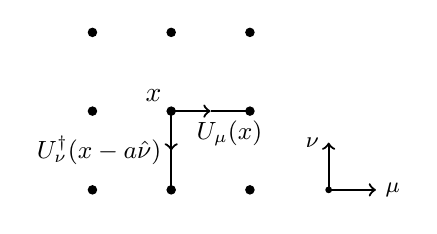
\begin{tikzpicture}
	\filldraw (0,0) circle (1.5pt);
	\filldraw (1,0) circle (1.5pt);
	\filldraw (2,0) circle (1.5pt);
	\filldraw (0,1) circle (1.5pt);
	\filldraw (1,1) circle (1.5pt);
	\filldraw (2,1) circle (1.5pt);
	\filldraw (0,2) circle (1.5pt);
	\filldraw (1,2) circle (1.5pt);
	\filldraw (2,2) circle (1.5pt);

	\draw [thick, ->] (1,1) -- (1.5,1);
	\draw [thick] (1.5,1) -- (2,1);
	\draw [thick, ->] (1,1) -- (1,0.5);
	\draw [thick] (1,0.5) -- (1,0);
	
	\filldraw (3,0) circle (1pt);
	\draw [thick, ->] (3,0) -- (3,0.6);
	\draw [thick, ->] (3,0) -- (3.6,0);
	\node[left] at (3,0.6) {\footnotesize $\nu$};
	\node[right] at (3.6,0) {\footnotesize $\mu$};

	\node[below right] at (1.2,1) {\small $U_\mu(x)$};
	\node[left] at (1,0.5) {\small $U^\dagger_\nu(x-a\hat{\nu})$};
	\node[above left] at (1,1) {$x$};
\end{tikzpicture}
\caption{Two link variables on the $\mu\nu$ plane. Reverse directions are represented by the inverse of the link variable.} \label{fig:LinkVar}
\end{figure}

The simplest path that can be created is the plaquette as shown in figure \ref{fig:Plaq}. Mathematically, this can be written as
\begin{align}
	P_{\mu\nu}=\frac{1}{3}\Re\Trace(U_\mu(x)U\nu(x+a\hat{\mu})U_\mu^\dagger(x+a\hat{\nu})U_\nu^\dagger(x)).
	\label{eq:Plaq}
\end{align}

\begin{figure}[h]
\centering
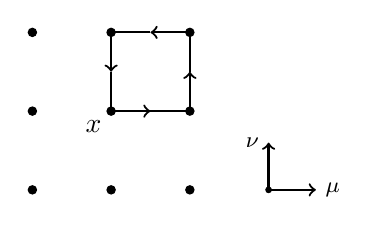
\begin{tikzpicture}
	\filldraw (0,0) circle (1.5pt);
	\filldraw (1,0) circle (1.5pt);
	\filldraw (2,0) circle (1.5pt);
	\filldraw (0,1) circle (1.5pt);
	\filldraw (1,1) circle (1.5pt);
	\filldraw (2,1) circle (1.5pt);
	\filldraw (0,2) circle (1.5pt);
	\filldraw (1,2) circle (1.5pt);
	\filldraw (2,2) circle (1.5pt);
	
	\draw [thick, ->] (1,1) -- (1.5,1);	\draw [thick] (1.5,1) -- (2,1);
	\draw [thick, ->] (2,1) -- (2,1.5);	\draw [thick] (2,1.5) -- (2,2);
	\draw [thick, ->] (2,2) -- (1.5,2);	\draw [thick] (1.5,2) -- (1,2);
	\draw [thick, ->] (1,2) -- (1,1.5);	\draw [thick] (1,1.5) -- (1,1);
	
	\filldraw (3,0) circle (1pt);
	\draw [thick, ->] (3,0) -- (3,0.6);
	\draw [thick, ->] (3,0) -- (3.6,0);
	\node[left] at (3,0.6) {\footnotesize $\nu$};
	\node[right] at (3.6,0) {\footnotesize $\mu$};

	\node[below left] at (1,1) {$x$};
\end{tikzpicture}
\caption{The plaquette which is the simplest guage invariant object that can be created from the link variables.} \label{fig:Plaq}
\end{figure}
With this, the Wilson gauge action is
\begin{align}
	S=\beta\sum_x\sum_{\mu>\nu}[1-P_{\mu\nu}(x)]
	\label{eq:WilsonAction}
\end{align}
where $\beta=6/g^2$ is the lattice coupling. The Wilson action is base on Wilson loops where the plaquette is an example of the simplest Wilson loop. It is the normalized ordered product of links in a path. It's used in equation \ref{eq:WilsonAction} and will be used in the improved action derived shortly. For small $a$, if we expand the plaquette at some $x_0$ as a polynomial in $a$, due to $A_\mu$ being slowly varying because $a$ is small, we find
\begin{align}
	P_{\mu\nu}=1-\frac{a^4}{6}\Trace(gF_\mu\nu(x_0))^2+\mathcal{O}(a^6)
\end{align}
where $F_{\mu\nu}=\partial_\mu A_\nu-\partial_\nu A_\mu+ig[A_\mu,A_\nu]$ is the field strength tensor. Taking the continuum limit $a\to0$, what remains is the continuum action up to second-order shown in equation \ref{eq:ContAction}.
\begin{align}
	S=\int\dd[4]{x}\frac{1}{2}\sum_{\mu,\nu}\Trace F_{\mu\nu}^2(x)
	\label{eq:ContAction}
\end{align}
These higher-order terms complicate the action as such:
\begin{align}
	S=\int\dd[4]{x}\sum_{\mu,\nu}\left[\frac{1}{2}\Trace F_{\mu\nu}^2(x)+\frac{a^2}{24}\Trace F_{\mu\nu}(D_\mu^2+D_\nu^2)F_{\mu\nu}+\ldots\right]
\end{align}
The terms $D_\mu$ and $D_\nu$ are gauge covariant derivatives for their respective directions.

To cancel out the higher-order term, we can introduce the rectangle operator. Similar to the plaquette in equation \ref{eq:Plaq}, it is the normalized real trace of the path in figure \ref{fig:Rect}.
\begin{figure}[h]
\centering
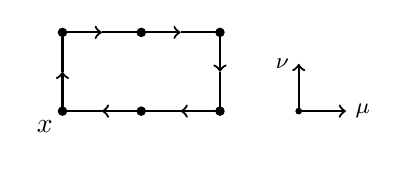
\begin{tikzpicture}
	\filldraw (0,0) circle (1.5pt);
	\filldraw (1,0) circle (1.5pt);
	\filldraw (2,0) circle (1.5pt);
	\filldraw (0,1) circle (1.5pt);
	\filldraw (1,1) circle (1.5pt);
	\filldraw (2,1) circle (1.5pt);
	
	\draw [thick, ->] (0,0) -- (0,0.5); \draw [thick] (0,0.5) -- (0,1);
	\draw [thick, ->] (0,1) -- (0.5,1); \draw [thick] (0.5,1) -- (1,1);
	\draw [thick, ->] (1,1) -- (1.5,1); \draw [thick] (1.5,1) -- (2,1);	
	\draw [thick, ->] (2,1) -- (2,0.5); \draw [thick] (2,0.5) -- (2,0);
	\draw [thick, ->] (2,0) -- (1.5,0); \draw [thick] (1.5,0) -- (1,0);
	\draw [thick, ->] (1,0) -- (0.5,0); \draw [thick] (0.5,0) -- (0,0);

	\filldraw (3,0) circle (1pt);
	\draw [thick, ->] (3,0) -- (3,0.6);
	\draw [thick, ->] (3,0) -- (3.6,0);
	\node[left] at (3,0.6) {\footnotesize $\nu$};
	\node[right] at (3.6,0) {\footnotesize $\mu$};

	\node[below left] at (0,0) {$x$};
\end{tikzpicture}
\caption{The rectangle operator at point $x$.} \label{fig:Rect}
\end{figure}
The rectangle operator has as an expansion
\begin{align}
	R_{\mu\nu}=1-\frac{4a^4}{6}\Trace(gF_{\mu\nu})^2-\frac{4a^6}{72}\Trace(gF_{\mu\nu}(4D_\mu^2+D_\nu^2)gF_{\mu\nu})+\mathcal{O}(a^8).
\end{align}
With the different coefficients for the $a^4$ and $a^6$ terms, an improved action can be calculated which is accurate up to third-order:
\begin{align}
	S_{imp}=-\beta\sum_x\sum_{\mu>\nu}\left[\frac{5}{3}P_{\mu\nu}-\frac{1}{12}(R_{\mu\nu}+R_{\nu\mu})\right].
	\label{eq:ImpAct}
\end{align}
One last modification to the above action is necessary for an accurate quantum action, that is an action that can accurately describe this system. This is the tadpole improvement, a renormalization $\mu_0$ that accounts for the extra terms in the action. Then equation \ref{eq:ImpAct} becomes
\begin{align}
	S_{imp}=-\beta\sum_x\sum_{\mu>\nu}\left[\frac{5}{3\mu_0^4}P_{\mu\nu}-\frac{1}{12\mu_0^6}(R_{\mu\nu}+R_{\nu\mu})\right]
	\label{eq:ImpActTPI}
\end{align}
where the $\mu_0$'s cancel the tadpole contributions. The $\mu_0$'s depend only on the lattice spacing and can be found numerically; for example, for a lattice spacing of $a=0.4$ fm, then $\mu_0\approx3/4$. In this case, the contribution by the rectangle operators is increased by about a factor of 2 compared to the action without the tadpole improvement. With the action in equation \ref{eq:ImpActTPI}, Monte Carlo steps can be used to run this model.

\subsection{Monte Carlo Application}
Again, the steps of Monte Carlo in this context is analogous to before. There are added complications that must be sorted out and, in doing so, increase the computing time appreciably. As stated before, the lattice is four-dimensional to account for three spacial dimensions and one temporal dimension. Furthermore, the calculations for the model exist at the links of which each lattice site has four.

We begin by looking at an $N$x$N$x$N$x$N$ lattice with coordinates $(x,\ y,\ z,\ t)$ at the site $x$ and the link in the $\hat{x}$ direction\footnote{In the code, the variable $n\in\{0,1,2,3\}$ is used to determine the specific link. This follows more easily with the sum in the action that is over $\mu>\nu$, thus $n_x=0\Leftrightarrow\hat{x}$, $n_y=1\Leftrightarrow\hat{y}$, etc.}. There are six plaquettes and twelve rectangle operators that affect the link $U_x(x)$ but for now we will focus only on the plaquettes. Figure \ref{fig:XPlane} shows these plaquettes. The plaquettes are equivalent for each plane that $U_x(x)$ is found on and the $yz$, $yt$ and $zt$ planes are not included (even though they are part of the sum in equation \ref{eq:ImpActTPI}) because they do not contain plaquettes of $U_x(x)$ and therefore do not contribute to the action for this link. So for any link, three of the planes will not contribute. It is important to note that each plane has a contribution of $U_\mu(x)$ and of $U_\mu^\dagger(x)$ for some $\mu$-direction.

\begin{figure}[h]
\centering
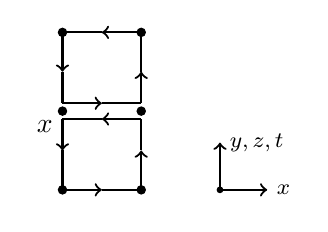
\begin{tikzpicture}
	\filldraw (0,0) circle (1.5pt);
	\filldraw (1,0) circle (1.5pt);
	\filldraw (0,1) circle (1.5pt);
	\filldraw (1,1) circle (1.5pt);
	\filldraw (0,2) circle (1.5pt);
	\filldraw (1,2) circle (1.5pt);
	
	\draw [thick, ->] (0,1.1) -- (0.5,1.1); \draw [thick] (0.5,1.1) -- (1,1.1);
	\draw [thick, ->] (1,1.1) -- (1,1.5); \draw [thick] (1,1.5) -- (1,2);
	\draw [thick, ->] (1,2) -- (0.5,2); \draw [thick] (0.5,2) -- (0,2);
	\draw [thick, ->] (0,2) -- (0,1.5); \draw [thick] (0,1.5) -- (0,1.1);
	
	\draw [thick, ->] (0,0.9) -- (0,0.5); \draw [thick] (0,0.5) -- (0,0);
	\draw [thick, ->] (0,0) -- (0.5,0); \draw [thick] (0.5,0) -- (1,0);
	\draw [thick, ->] (1,0) -- (1,0.5); \draw [thick] (1,0.5) -- (1,0.9);
	\draw [thick, ->] (1,0.9) -- (0.5,0.9); \draw [thick] (0.5,0.9) -- (0,0.9);

	\filldraw (2,0) circle (1pt);
	\draw [thick, ->] (2,0) -- (2,0.6);
	\draw [thick, ->] (2,0) -- (2.6,0);
	\node[right] at (2,0.6) {\footnotesize $y,z,t$};
	\node[right] at (2.6,0) {\footnotesize $x$};

	\node[below left] at (0,1) {$x$};
\end{tikzpicture}
\caption{Two plaquettes that effect the link $U_x(x)$ with one being the inverse path or $U_x^\dagger(x)$. Since the lattice is four dimensional, the three planes of $x$ are analogous for calculation of $U_x(x)$.} \label{fig:XPlane}
\end{figure}

The picture for $U_t(x)$ is slightly different. Because $n_t>n_i$ for all $i\in\{x,y,z\}$, the plaquette at site $x$ contains the inverse link of $U_t(x)$. Thus the plaquette at site $x-a\hat{\mu}$ must be used as the plaquette containing $U_t(x)$ as shown in figure \ref{fig:TPlane}. For links in the $t$-direction, this is always true while for links in the $x$-direction, this is never true. The application of this can be seen in the code in figure \ref{fig:ComputePlaqStaples} which will be discribed shortly.

\begin{figure}[h]
\centering
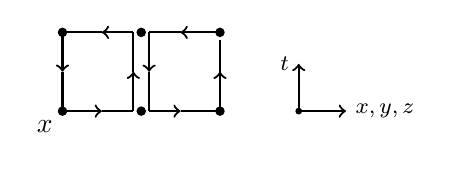
\begin{tikzpicture}
	\filldraw (0,0) circle (1.5pt);
	\filldraw (1,0) circle (1.5pt);
	\filldraw (2,0) circle (1.5pt);
	\filldraw (0,1) circle (1.5pt);
	\filldraw (1,1) circle (1.5pt);
	\filldraw (2,1) circle (1.5pt);
	
	\draw [thick, ->] (0,0) -- (0.5,0); \draw [thick] (0.5,0) -- (0.9,0);
	\draw [thick, ->] (0.9,0) -- (0.9,0.5); \draw [thick] (0.9,0.5) -- (0.9,1);
	\draw [thick, ->] (0.9,1) -- (0.5,1); \draw [thick] (0.5,1) -- (0,1);
	\draw [thick, ->] (0,1) -- (0,0.5); \draw [thick] (0,0.5) -- (0,0);
	
	\draw [thick, ->] (1.1,1) -- (1.1,0.5); \draw [thick] (1.1,0.5) -- (1.1,0);
	\draw [thick, ->] (1.1,0) -- (1.5,0); \draw [thick] (1.5,0) -- (2,0);
	\draw [thick, ->] (2,0) -- (2,0.5); \draw [thick] (2,0.5) -- (2,0.9);
	\draw [thick, ->] (2,1) -- (1.5,1); \draw [thick] (1.5,1) -- (1.1,1);

	\filldraw (3,0) circle (1pt);
	\draw [thick, ->] (3,0) -- (3,0.6);
	\draw [thick, ->] (3,0) -- (3.6,0);
	\node[left] at (3,0.6) {\footnotesize $t$};
	\node[right] at (3.6,0) {\footnotesize $x,y,z$};

	\node[below left] at (0,0) {$x$};
\end{tikzpicture}
\caption{Two plaquettes that effect the link $U_t(x)$. This picture holds for the planes where $\mu>\nu$.} \label{fig:TPlane}
\end{figure}

The rectangle operators are analogous but there is one important difference. Since these operators are $a\cross2a$ and not $a\cross a$ as are the plaquettes, there are more contributions to the operator. This can be seen in figure \ref{fig:RectOp}. As with the plaquette, the paths in this figure are for the $x$-direction but these paths will not be so for the $t$-direction. Rather, there is a rotation as before and for the same reason. Also, from equation \ref{eq:ImpActTPI}, there are terms $R_{\mu\nu}$ and $R_{\nu\mu}$. Thus there are six rectangle operators, double the number of plaquettes. For $U_x(x)$, there are only two staples for $R_{\nu\mu}$ and four for $R_{\mu\nu}$ and vis versa for $U_t(x)$. The staple being defined as the path operator without the path link in question. To sum up, if $n_\mu>n_\nu$, then $R_{\mu\nu}$ will be a sum of four staples and $R_{\nu\mu}$ will be the sum of two.
\begin{figure}[h]
\centering
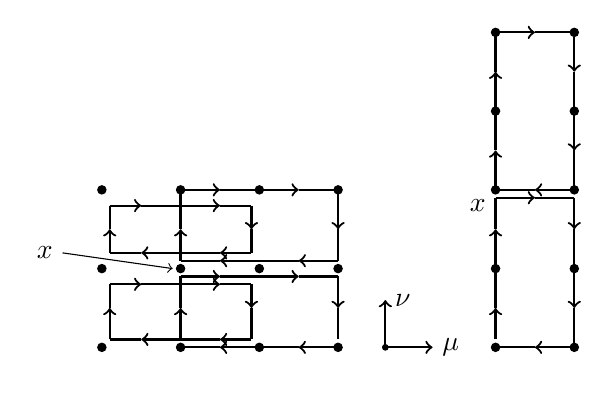
\begin{tikzpicture}
	\filldraw (0,0) circle (1.5pt);
	\filldraw (1,0) circle (1.5pt);
	\filldraw (2,0) circle (1.5pt);
	\filldraw (3,0) circle (1.5pt);
	\filldraw (0,1) circle (1.5pt);
	\filldraw (1,1) circle (1.5pt);
	\filldraw (2,1) circle (1.5pt);
	\filldraw (3,1) circle (1.5pt);
	\filldraw (0,2) circle (1.5pt);
	\filldraw (1,2) circle (1.5pt);
	\filldraw (2,2) circle (1.5pt);
	\filldraw (3,2) circle (1.5pt);

	\filldraw (5,0) circle (1.5pt);
	\filldraw (6,0) circle (1.5pt);
	\filldraw (5,1) circle (1.5pt);
	\filldraw (6,1) circle (1.5pt);
	\filldraw (5,2) circle (1.5pt);
	\filldraw (6,2) circle (1.5pt);
	\filldraw (5,3) circle (1.5pt);
	\filldraw (6,3) circle (1.5pt);
	\filldraw (5,4) circle (1.5pt);
	\filldraw (6,4) circle (1.5pt);
	
	\draw [thick, ->] (1,1.1) -- (1,1.5); \draw [thick] (1,1.5) -- (1,2);
	\draw [thick, ->] (1,2) -- (1.5,2); \draw [thick] (1.5,2) -- (2,2);
	\draw [thick, ->] (2,2) -- (2.5,2); \draw [thick] (2.5,2) -- (3,2);	
	\draw [thick, ->] (3,2) -- (3,1.5); \draw [thick] (3,1.5) -- (3,1.1);
	\draw [thick, ->] (3,1.1) -- (2.5,1.1); \draw [thick] (2.5,1.1) -- (2,1.1);
	\draw [thick, ->] (2,1.1) -- (1.5,1.1); \draw [thick] (1.5,1.1) -- (1,1.1);
	
	\draw [thick, ->] (1,0.1) -- (1,0.5); \draw [thick] (1,0.5) -- (1,0.9);
	\draw [thick, ->] (1,0.9) -- (1.5,0.9); \draw [thick] (1.5,0.9) -- (2,0.9);
	\draw [thick, ->] (2,0.9) -- (2.5,0.9); \draw [thick] (2.5,0.9) -- (3,0.9);	
	\draw [thick, ->] (3,0.9) -- (3,0.5); \draw [thick] (3,0.5) -- (3,0.1);
	\draw [thick, ->] (3,0) -- (2.5,0); \draw [thick] (2.5,0) -- (2,0);
	\draw [thick, ->] (2,0) -- (1.5,0); \draw [thick] (1.5,0) -- (1,0);
	
	\draw [thick, ->] (0.1,1.2) -- (0.1,1.5); \draw [thick] (0.1,1.5) -- (0.1,1.8);
	\draw [thick, ->] (0.1,1.8) -- (0.5,1.8); \draw [thick] (0.5,1.8) -- (0.9,1.8);
	\draw [thick, ->] (0.9,1.8) -- (1.5,1.8); \draw [thick] (1.5,1.8) -- (1.9,1.8);	
	\draw [thick, ->] (1.9,1.8) -- (1.9,1.5); \draw [thick] (1.9,1.5) -- (1.9,1.2);
	\draw [thick, ->] (1.9,1.2) -- (1.5,1.2); \draw [thick] (1.5,1.2) -- (0.9,1.2);
	\draw [thick, ->] (0.9,1.2) -- (0.5,1.2); \draw [thick] (0.5,1.2) -- (0.1,1.2);	

	\draw [thick, ->] (0.1,0.1) -- (0.1,0.5); \draw [thick] (0.1,0.5) -- (0.1,0.8);
	\draw [thick, ->] (0.1,0.8) -- (0.5,0.8); \draw [thick] (0.5,0.8) -- (0.9,0.8);
	\draw [thick, ->] (0.9,0.8) -- (1.5,0.8); \draw [thick] (1.5,0.8) -- (1.9,0.8);	
	\draw [thick, ->] (1.9,0.8) -- (1.9,0.5); \draw [thick] (1.9,0.5) -- (1.9,0.1);
	\draw [thick, ->] (1.9,0.1) -- (1.5,0.1); \draw [thick] (1.5,0.1) -- (0.9,0.1);
	\draw [thick, ->] (0.9,0.1) -- (0.5,0.1); \draw [thick] (0.5,0.1) -- (0.1,0.1);		
	
	\draw [thick, ->] (5,0.1) -- (5,0.5); \draw [thick] (5,0.5) -- (5,1);
	\draw [thick, ->] (5,1) -- (5,1.5); \draw [thick] (5,1.5) -- (5,1.9);
	\draw [thick, ->] (5,1.9) -- (5.5,1.9); \draw [thick] (5.5,1.9) -- (6,1.9);
	\draw [thick, ->] (6,1.9) -- (6,1.5); \draw [thick] (6,1.5) -- (6,1);
	\draw [thick, ->] (6,1) -- (6,0.5); \draw [thick] (6,0.5) -- (6,0);
	\draw [thick, ->] (6,0) -- (5.5,0); \draw [thick] (5.5,0) -- (5,0);
	
	\draw [thick, ->] (5,2) -- (5,2.5); \draw [thick] (5,2.5) -- (5,3);
	\draw [thick, ->] (5,3) -- (5,3.5); \draw [thick] (5,3.5) -- (5,4);
	\draw [thick, ->] (5,4) -- (5.5,4); \draw [thick] (5.5,4) -- (6,4);
	\draw [thick, ->] (6,4) -- (6,3.5); \draw [thick] (6,3.5) -- (6,3);
	\draw [thick, ->] (6,3) -- (6,2.5); \draw [thick] (6,2.5) -- (6,2);
	\draw [thick, ->] (6,2) -- (5.5,2); \draw [thick] (5.5,2) -- (5,2);
	
	\filldraw (3.6,0) circle (1pt);
	\draw[thick, ->] (3.6,0) -- (3.6,0.6);
	\draw[thick, ->] (3.6,0) -- (4.2,0);
	\node[right] at (3.6,0.6) {$\nu$};
	\node[right] at (4.2,0) {$\mu$};
	
	\node[below left] at (5,2) {$x$};
	\draw[->] (-0.5,1.2) -- (0.9,1);
	\node[left] at (-0.5,1.2) {$x$};
\end{tikzpicture}
\caption{The possible configurations of the rectangle operator. Depending on the direction, the rectangles may be rotated as with the plaquettes. For $U_t(x)$, the rectangles are rotated 90$^\circ$ relative to $U_x(x)$.} \label{fig:RectOp}
\end{figure}

In the code in \ref{fig:ComputePlaqStaples}, the function \texttt{nPlaq} calculates the staple and conjugate staple for the link at lattice site $(x,\ y,\ z,\ t,\ n)$ where $n$ specifies the link. The values \texttt{staples} and \texttt{stapleC} are the sums of the staples and conjugate staples, respectively. They are used to calculate $\Delta S$ (along with the rectangle staples for the improved action).
\begin{figure}[h]
\begin{lstlisting}
def nPlaq(x, y, z, t, n):
    a = [0] * 4
    a[n] = 1
    staples = 0
    stapleC = 0

    for i in range(3 - n):
        staples += mm(L[m(x+a[0])][m(y+a[1])][m(z+a[2])][t][n+i+1],
                        ct(L[x][m(y+a[-i])][m(z+a[1-i])][m(t+a[2-i])][n]),
                        ct(L[x][y][z][t][n+i+1]))
        stapleC += mm(ct(L[x][m(y-a[-i])][m(z-a[1-i])][m(t-a[2-i])][n+i+1]),
                        L[x][m(y-a[-i])][m(z-a[1-i])][m(t-a[2-i])][n],
                        L[m(x+a[0])][m(y+a[1]-a[-i])][m(z+a[2]-a[1-i])][t-a[2-i]][n+i+1])
    for i in range(n):
        staples += mm(ct(L[m(x-a[i+n])][m(y-a[i+n-1]+a[1])][m(z-a[i+n-2]+a[2])][m(t+a[3])][i]),
                        ct(L[m(x-a[i+n])][m(y-a[i+n-1])][m(z-a[i+n-2])][t][n]),
                        L[m(x-a[i+n])][m(y-a[i+n-1])][m(z-a[i+n-2])][t][i])
        stapleC += mm(L[x][y][z][t][i],
                        L[m(x+a[i+n])][m(y+a[i+n-1])][m(z+a[i+n-2])][t][n],
                        ct(L[x][m(y+a[1])][m(z+a[2])][m(t+a[3])][i]))
    return staples, stapleC
\end{lstlisting}
\caption{Python code for calculating the regular and conjugate transpose staples for $U_\mu(x)$, a link in direction $n_\mu$. The two for loops are to account for the change in the calculation of the staples for each link direction.}
\label{fig:ComputePlaqStaples}
\end{figure}

In the previous model, a small random change $\epsilon$ was added to a time slice for a path $x$ and the resulting change in the action was calculated. The same is done again except the path links are $SU(3)$ matrices, not numbers, so a `small' random $SU(3)$ matrix is added to the path link, that is a matrix close to the identity. Thus we take $U\to MU$ if $U$ is a path link and $M\in SU(3)$ is close to the identity. The small change in $U$ is given by the product $MU$ which is also an $SU(3)$ matrix since $SU(3)$ is a group and thus is closed under this operation. This resulting change is used to calculate the change in the action, $\Delta S$.

Let $\mathcal{S}_{\mu\nu}(C)$ represent the staple(s)\footnote{Here I say ``staple(s)" because there can be more than one staple coming from the $\mu\nu$ plane like with the rectangle operator (where there can be two). It is implied these are being summed first in the equation which is more useful as a template for visualizing $\Delta S$ than a rigorous formula.} for $U_\mu(x)$ in the $\mu\nu$ plane for path $C$ and $\mathcal{S}^*_{\mu\nu}(C)$ be the staple(s) for $U_\mu^\dagger(x)$. Then the change in the unimproved action from equation \ref{eq:WilsonAction} for site $x$ is
\begin{align}
	\Delta S(x)=\frac{\beta}{3}\Re\Trace\left[(I-M)U_\mu(x)\sum_{\nu\neq\mu}\mathcal{S}_{\mu\nu}(P_{\mu\nu})+U^\dagger_\mu(x)(I-M^\dagger)\sum_{\nu\neq\mu}\mathcal{S}^*_{\mu\nu}(P_{\mu\nu})\right]
	\label{eq:MCNormAction}
\end{align}
and the improved action is
\begin{align}
\begin{split}
	\Delta S_{imp}(x)=\frac{\beta}{3}\Re\Trace\left[(I-M)U_\mu(x)\left(c_1\sum_{\nu\neq\mu}\mathcal{S}_{\mu\nu}(P_{\mu\nu})-c_2\sum_{\nu\neq\mu}[\mathcal{S}_{\mu\nu}(R_{\mu\nu})+\mathcal{S}_{\mu\nu}(R_{\nu\mu})]\right)\right.\\
	\left.+U^\dagger_\mu(x)(I-M^\dagger)\left(c_1\sum_{\nu\neq\mu}\mathcal{S}^*_{\mu\nu}(P_{\mu\nu})-c^2\sum_{\nu\neq\mu}[\mathcal{S}^*_{\mu\nu}(R_{\mu\nu})+\mathcal{S}^*_{\mu\nu}(R_{\nu\mu})\right)\right]
\end{split}
	\label{eq:MCImpAction}
\end{align}
where $M$ is a random $SU(3)$ matrix close to the identity, $c_1=5/3\mu_0^4$ and $c_2=1/12\mu_0^6$. With this in mind, one sweep of the lattice can be completed with the following steps:
\begin{enumerate}
\item Choose a site $x$ and a link $n$.
\item Choose a random $SU(3)$ matrix $M$ such that $U_\mu(x)\to MU_\mu(x)$.
\item Calculate the change in action $\Delta S$ with equation \ref{eq:MCImpAction}.
\item If $\Delta S<0$, then keep the change $MU_\mu(x)$.
\item Otherwise assign it a probability $\exp(-\Delta S)$ of changing.
\item Repeat steps 1-5 for every site on the path.
\end{enumerate}
\begin{figure}[h]
\begin{lstlisting}
def dS(staples, stapleC, rects, rectC, x, y, z, t, n):
    M = SU3list[np.random.randint(0, 2 * numMatrices)]
    U = L[x][y][z][t][n]
    deltaS = (beta / 3) * np.real(np.trace(np.dot(U - mm(M, U), c1 * staples - c2 * rects) + \
                                        np.dot(ct(U) - ct(mm(M, U)), c1 * stapleC - c2 * rectC)))             
    return deltaS, M

def sweep():
    for p in product(range(N), range(N), range(N), range(N), range(4)):
        x, y, z, t, n = p
        staples, stapleC = nPlaq(x, y, z, t, n)
        rects, rectC = nRect(x,y,z,t,n)
        for _ in range(N_ma):
            deltaS, M = dS(staples, stapleC, rects, rectC, x, y, z, t, n)
            if deltaS < 0 or np.random.random() < np.exp(-deltaS):
                L[x][y][z][t][n] = np.dot(M, L[x][y][z][t][n])
\end{lstlisting}
\caption{The code that evolves the lattice. The array \texttt{L} is the lattice with $N^4*4$ sites given $N$ as the side length of the lattice and an $SU(3)$ matrix at each site with the total length of \texttt{L} being $36*N^4$. The function \texttt{sweep} completes a sweep of the lattice and \texttt{dS} calculates the change in the action. At each site $(x,\ y,\ z,\ t,\ n)$, the Metropolis algorithm is done \texttt{N\_ma} times so as to let the link variable reach an equilibrium with its neighbors before moving on to the next link.}
\label{fig:LQCDSweep}
\end{figure}

These steps are very similar to those from before, the main changes coming in the equation for the action which is much more costly in this model; the lattice is higher dimensional and the Monte Carlo steps require more computations and are computed on matrices. In figure \ref{fig:LQCDSweep}, equation \ref{eq:MCImpAction} is implemented under \texttt{dS} where the matrices \text{staples} and \text{stapleC} are calculated as shown in figure \ref{fig:ComputePlaqStaples} and \texttt{rects} and \texttt{rectC} are calculated in a similar but longer function \texttt{nRect}. The $SU(3)$ matrices used as the small Monte Carlo variable are generated beforehand and stored in \texttt{SU3list} along with their inverses.

\subsection{Measurements}
With the derivation of the path integral in mind, we precede with the gluonic path integral similarly with $N=8$ as a lattice size\footnote{Even though this lattice size is much smaller than the previous, this simulation requires hours, compared to minutes, to complete 25 measurements with 50 sweeps between measurements. All code was run in Python 3.x on an Intel i7 processor on Windows 10.}. We can measure the effect of the Wilson loop operator on the vacuum state and, with the choice of Wilson loop, the measurement will change. First, the lattice is thermalized, as defined earlier, by completing 100 sweeps and then measurements are taken every $N_{cor}=50$ sweeps. The trace of the Wilson loops for each path link are summed and averaged. In figure \ref{fig:LQCDConv}, the convergence of the Wilson loops are shown. After 100 sweeps, the lattice has reach equilibrium and 50 sweeps is sufficiently long enough to prevent correlation in the measurements \cite{MainPaper}.

\begin{figure}[h]
	\centering
	\includegraphics[scale=0.60]{LQCD_Convergence.png}
	\caption{A visualization of the convergence rates of the Monte Carlo measurements. The first 100 sweeps, which are plotted, are used for reaching the equilibrium of the lattice and so measurements are not completed during these sweeps.}
	\label{fig:LQCDConv}
\end{figure}

The Monte Carlo averages of $a\cross a$, $a\cross2a$ and $a\cross3a$ Wilson loops are calculated as shown in the code in figure \ref{fig:LQCDMCCode}. In general, measurement of an arbitrary Wilson loop $W$ requires only a change in the product of the link variables.

The averages are also calculated for both the unimproved and improved actions:
\begin{align}
	S(x)=\frac{\beta}{\mu_0^4}\sum_{\mu>\nu}P_{\mu\nu}(x)\qquad\ S_{imp}(x)=-\beta\sum_{\mu>\nu}\left[\frac{5}{3\mu_0^4}P_{\mu\nu}-\frac{1}{12\mu_0^6}(R_{\mu\nu}+R_{\nu\mu})\right].
	\label{eq:ActAgain}
\end{align}
This allows us to visual the difference in the second- and third-order accuracy of the discretized action, i.e. the contribution of the rectangle operators. For the unimproved and improved actions, the averages, denoted by $\mathcal{W}$ and $\mathcal{W}_{imp}$, respectively, are
\begin{align}
\begin{split}
	\mathcal{W}(a\cross a)=0.497\pm0.003\qquad\quad&\mathcal{W}_{imp}(a\cross a)=0.546\pm0.003,\\
	\mathcal{W}(a\cross2a)=0.260\pm0.004\qquad\quad&\mathcal{W}_{imp}(a\cross2a)=0.290\pm0.004,\\
	\mathcal{W}(a\cross3a)=0.137\pm0.004\qquad\quad&\mathcal{W}_{imp}(a\cross3a)=0.156\pm0.003.
\end{split}
\end{align}
These are the unweighted means for the respective Wilson loops as shown in figure \ref{fig:LQCDMCCode}. These results suggest that the larger the area of the Wilson loop, the smaller $\mathcal{W}$ will be.
\begin{figure}[h!]
\begin{lstlisting}
def measure(loopLength):
    LAvg = 0
    for p in product(range(N), range(N), range(N), range(N)):
        x, y, z, t = p
        link = measureLink(x, y, z, t, loopLength)
        LAvg += np.real(np.trace( 
        mm(L[x][y][z][t][0], L[m(x+1)][y][z][t][1], link[0], ct(L[x][y][z][t][1])) + 
        mm(L[x][y][z][t][0], L[m(x+1)][y][z][t][2], link[1], ct(L[x][y][z][t][2])) + 
        mm(L[x][y][z][t][0], L[m(x+1)][y][z][t][3], link[2], ct(L[x][y][z][t][3])) + 
        mm(L[x][y][z][t][1], L[x][m(y+1)][z][t][2], link[3], ct(L[x][y][z][t][2])) + 
        mm(L[x][y][z][t][1], L[x][m(y+1)][z][t][3], link[4], ct(L[x][y][z][t][3])) + 
        mm(L[x][y][z][t][2], L[x][y][m(z+1)][t][3], link[5], ct(L[x][y][z][t][3]))))
    return LAvg / N**4 / 18
\end{lstlisting}
	\caption{Python code that measures an $a\cross ca$ Wilson loop for $c\in\{1,2,3\}$.}% The array \texttt{link} determines specific links in the loop based on \texttt{loopLength}. The returned value is the normalized average.}
	\label{fig:LQCDMCCode}
\end{figure}

\begin{figure}[h!]
	\centering
	\includegraphics[scale=0.60]{LQCD_MC_Measurements.png}
	\caption{Monte Carlo measurements for $a\cross a$, $a\cross2a$ and $a\cross3a$ Wilson loops. The triangles represent the improved action from equation \ref{eq:ImpActTPI} while the squares represent the unimproved action from equation \ref{eq:WilsonAction}. Between each measurement, $N_{cor}=50$ sweeps were omitted.}
	\label{fig:LQCDPlot}
\end{figure}

With the system modeled based on the assumptions of the system, the measurements are relatively trivial in both computational time and in the complexity of the code. Further measurements can be made on this lattice or more realistic properties can be assumed for the lattice, although the latter may increase the computing time significantly due to its added complexity. Nevertheless, as with the previous models, the potential for added measurements exists.

\section{Conclusion and Remarks}
In this paper, we explored the use of Monte Carlo techniques on physical models. I used the Python language because of my previous experiences with it and its convenience especially with mathematical operations, multidimensional arrays and useful libraries such as \texttt{numpy} and \texttt{matplotlib}. Going forward, implementing these models in a language such as C would be an advantageous endeavor since the flaw of Python is its inefficiency especially compared to C and C-like languages. Also, the use of a Message Passing Interface (MPI) and/or multithreading would also help with the time inconveniences faced with lattice QCD models. And with the lack of time, more significant measurements and more accurate lattice QCD models were not able to be explored as was hoped. As such, this may be a future project to expand on what I have learned thus far in lattice QCD.

That being said, we have seen the flexibility and power that some Monte Carlo methods have. The use of the Metropolis algorithm, assuming ergodicity and detailed balance, is extremely powerful because of its ability to converge on a desired equilibrium. And, due to taking a large sample size, possibly complex expectation values and measurements can be accurately approximated if simplified to a mean. As is shown in \cite{MainPaper}, for some functional $\Gamma[x]$ such that
\begin{align}
	\langle\Gamma[x]\rangle=\frac{\int\mathcal{D}[x(t)]\Gamma[x]e^{-S[x]}}{\int\mathcal{D}[x(t)]e^{-S[x]}},
\end{align}
we can instead approximate it by
\begin{align}
	\langle\Gamma[x]\rangle\approx\overline{\Gamma}\equiv\frac{1}{N}\sum_{i=1}^N\Gamma[x^{(\alpha)}]
\end{align}
if the probability for some path $x^{(\alpha)}$ is equal to the weight of the expectation value (in this case $e^{-S[x]}$. The above can be very easily computed in a program and the error comes just from the sample size $N$.

Also, this paper has yielded some satisfying results. The expectation of the magnetization and susceptibility in the Ising model was modeled successfully, as with the excitation energy $E_1-E_0$ of the harmonic oscillator. The latter can be solved by the Schr\"odinger equation but it was satisfying to see the same result through the use of Feynman path integrals and the Metropolis algorithm, a completely different approach. Lastly, three different Wilson loops, $a\cross a$, $a\cross2a$ and $a\cross3a$, were calculated using an improved Wilson action. Nevertheless, such a measurement is just the beginning; measurements such as a static quark, anti-quark potential and many others could next be calculated.

Important portions of the code I used in this paper have been are shown but the entirety of every program is too lengthy and cumbersome to add to this paper. So, all of the code used in this paper can be found on GitHub at:

\url{http://github.com/crumpstrr33/Monte-Carlo-Applications-and-Lattice-QCD}.

\break
\bibliographystyle{abbrv}
\bibliography{Citations}

\end{document}